\documentclass[12pt, a4paper,  BCOR=8.25mm, DIV=15]{scrartcl}\usepackage[]{graphicx}\usepackage[]{color}
%% maxwidth is the original width if it is less than linewidth
%% otherwise use linewidth (to make sure the graphics do not exceed the margin)
\makeatletter
\def\maxwidth{ %
  \ifdim\Gin@nat@width>\linewidth
    \linewidth
  \else
    \Gin@nat@width
  \fi
}
\makeatother

\definecolor{fgcolor}{rgb}{0.345, 0.345, 0.345}
\newcommand{\hlnum}[1]{\textcolor[rgb]{0.686,0.059,0.569}{#1}}%
\newcommand{\hlstr}[1]{\textcolor[rgb]{0.192,0.494,0.8}{#1}}%
\newcommand{\hlcom}[1]{\textcolor[rgb]{0.678,0.584,0.686}{\textit{#1}}}%
\newcommand{\hlopt}[1]{\textcolor[rgb]{0,0,0}{#1}}%
\newcommand{\hlstd}[1]{\textcolor[rgb]{0.345,0.345,0.345}{#1}}%
\newcommand{\hlkwa}[1]{\textcolor[rgb]{0.161,0.373,0.58}{\textbf{#1}}}%
\newcommand{\hlkwb}[1]{\textcolor[rgb]{0.69,0.353,0.396}{#1}}%
\newcommand{\hlkwc}[1]{\textcolor[rgb]{0.333,0.667,0.333}{#1}}%
\newcommand{\hlkwd}[1]{\textcolor[rgb]{0.737,0.353,0.396}{\textbf{#1}}}%

\usepackage{framed}
\makeatletter
\newenvironment{kframe}{%
 \def\at@end@of@kframe{}%
 \ifinner\ifhmode%
  \def\at@end@of@kframe{\end{minipage}}%
  \begin{minipage}{\columnwidth}%
 \fi\fi%
 \def\FrameCommand##1{\hskip\@totalleftmargin \hskip-\fboxsep
 \colorbox{shadecolor}{##1}\hskip-\fboxsep
     % There is no \\@totalrightmargin, so:
     \hskip-\linewidth \hskip-\@totalleftmargin \hskip\columnwidth}%
 \MakeFramed {\advance\hsize-\width
   \@totalleftmargin\z@ \linewidth\hsize
   \@setminipage}}%
 {\par\unskip\endMakeFramed%
 \at@end@of@kframe}
\makeatother

\definecolor{shadecolor}{rgb}{.97, .97, .97}
\definecolor{messagecolor}{rgb}{0, 0, 0}
\definecolor{warningcolor}{rgb}{1, 0, 1}
\definecolor{errorcolor}{rgb}{1, 0, 0}
\newenvironment{knitrout}{}{} % an empty environment to be redefined in TeX

\usepackage{alltt}
\usepackage[utf8]{inputenc}
\usepackage{newfloat}
\DeclareFloatingEnvironment[name={Supplementary Figure}]{suppfigure}

\newenvironment{itemizz}%
  {\begin{itemize}%
    \setlength{\itemsep}{2pt}%
    \setlength{\parskip}{2pt}}%
  {\end{itemize}}

\newcommand{\txtt}[1]{{\texttt{#1}}}
\IfFileExists{upquote.sty}{\usepackage{upquote}}{}
\begin{document}
%\VignetteEngine{knitr::knitr}
%\VignetteIndexEntry{Map Overlays  and Spatial Modeling (Set 13)}



\title{13: Map Overlays  and Spatial Modeling}
\author{John H Maindonald}
\maketitle

\vspace*{-0.5cm}
\begin{knitrout}
\definecolor{shadecolor}{rgb}{0.969, 0.969, 0.969}\color{fgcolor}\begin{kframe}
\begin{alltt}
\hlstd{doFigs} \hlkwb{<-} \hlnum{TRUE}
\end{alltt}
\end{kframe}
\end{knitrout}
\vspace*{-0.5cm}

Start by attaching required packages:

\begin{knitrout}
\definecolor{shadecolor}{rgb}{0.969, 0.969, 0.969}\color{fgcolor}\begin{kframe}
\begin{alltt}
\hlstd{figset13} \hlkwb{<-} \hlkwa{function}\hlstd{()\{}
  \hlkwa{if}\hlstd{(}\hlopt{!}\hlkwd{requireNamespace}\hlstd{(}\hlstr{'DAAG'}\hlstd{,} \hlkwc{quietly} \hlstd{=} \hlnum{TRUE}\hlstd{))}\hlkwd{stop}\hlstd{(}\hlstr{'DAAG must be installed'}\hlstd{)}
  \hlkwa{if}\hlstd{(}\hlopt{!}\hlkwd{require}\hlstd{(}\hlstr{'latticeExtra'}\hlstd{,} \hlkwc{quietly} \hlstd{=} \hlnum{TRUE}\hlstd{))}\hlkwd{stop}\hlstd{(}\hlstr{'latticeExtra must be installed'}\hlstd{)}
  \hlkwa{if}\hlstd{(}\hlopt{!}\hlkwd{requireNamespace}\hlstd{(}\hlstr{'oz'}\hlstd{,} \hlkwc{quietly} \hlstd{=} \hlnum{TRUE}\hlstd{))}\hlkwd{stop}\hlstd{(}\hlstr{'oz must be installed'}\hlstd{)}
  \hlkwa{if}\hlstd{(}\hlopt{!}\hlkwd{requireNamespace}\hlstd{(}\hlstr{'rgdal'}\hlstd{,} \hlkwc{quietly}\hlstd{=}\hlnum{TRUE}\hlstd{))}\hlkwd{stop}\hlstd{(}\hlstr{'rgdal must be installed'}\hlstd{)}
  \hlkwa{if}\hlstd{(}\hlopt{!}\hlkwd{require}\hlstd{(}\hlstr{'sp'}\hlstd{,} \hlkwc{quietly} \hlstd{=} \hlnum{TRUE}\hlstd{))}\hlkwd{stop}\hlstd{(}\hlstr{'sp must be installed'}\hlstd{)}
  \hlstd{\}}
\end{alltt}
\end{kframe}
\end{knitrout}

\begin{knitrout}
\definecolor{shadecolor}{rgb}{0.969, 0.969, 0.969}\color{fgcolor}\begin{kframe}
\begin{alltt}
\hlkwd{figset13}\hlstd{()}
\end{alltt}
\end{kframe}
\end{knitrout}

\begin{knitrout}
\definecolor{shadecolor}{rgb}{0.969, 0.969, 0.969}\color{fgcolor}\begin{kframe}
\begin{alltt}
\hlstd{fig13.1} \hlkwb{<-} \hlkwa{function}\hlstd{()\{}
\hlcom{## ---- oz-sites ----}
\hlstd{oz}\hlopt{::}\hlkwd{oz}\hlstd{(}\hlkwc{sections}\hlstd{=}\hlkwd{c}\hlstd{(}\hlnum{3}\hlopt{:}\hlnum{5}\hlstd{,} \hlnum{11}\hlopt{:}\hlnum{16}\hlstd{),} \hlkwc{col}\hlstd{=}\hlstr{"gray"}\hlstd{)}
\hlstd{chh} \hlkwb{<-} \hlkwd{par}\hlstd{()}\hlopt{$}\hlstd{cxy[}\hlnum{2}\hlstd{]}
\hlkwd{with}\hlstd{(DAAG}\hlopt{::}\hlstd{possumsites, \{}
  \hlkwd{points}\hlstd{(Longitude,}
         \hlstd{Latitude}\hlopt{+}\hlkwd{c}\hlstd{(}\hlnum{0}\hlstd{,}\hlnum{0}\hlstd{,}\hlnum{0}\hlstd{,}\hlnum{.2}\hlstd{,}\hlopt{-}\hlnum{.2}\hlstd{,} \hlnum{0}\hlstd{,}\hlnum{0}\hlstd{)}\hlopt{*}\hlstd{chh,}
         \hlkwc{col}\hlstd{=}\hlstr{"blue"}\hlstd{)}
  \hlkwd{text}\hlstd{(Latitude} \hlopt{~} \hlstd{Longitude,}
       \hlkwc{labels}\hlstd{=}\hlkwd{rownames}\hlstd{(DAAG}\hlopt{::}\hlstd{possumsites),}
       \hlkwc{col}\hlstd{=}\hlstr{"red"}\hlstd{,} \hlkwc{pos}\hlstd{=}\hlkwd{c}\hlstd{(}\hlnum{2}\hlstd{,}\hlnum{4}\hlstd{,}\hlnum{2}\hlstd{,}\hlnum{1}\hlstd{,}\hlnum{3}\hlstd{,}\hlnum{2}\hlstd{,}\hlnum{2}\hlstd{),} \hlkwc{xpd}\hlstd{=}\hlnum{TRUE}\hlstd{)}
  \hlcom{# pos = 1:below, 2:left, 3:above, 4:right}
  \hlcom{# xpd=TRUE allows plotting outside figure region}
\hlstd{\})}
\hlstd{\}}
\end{alltt}
\end{kframe}
\end{knitrout}

\begin{figure}
\begin{knitrout}
\definecolor{shadecolor}{rgb}{0.969, 0.969, 0.969}\color{fgcolor}\begin{kframe}
\begin{alltt}
\hlstd{opar} \hlkwb{<-} \hlkwd{par}\hlstd{(}\hlkwc{mar}\hlstd{=}\hlkwd{c}\hlstd{(}\hlnum{4}\hlstd{,}\hlnum{4}\hlstd{,}\hlnum{1.6}\hlstd{,}\hlnum{3.1}\hlstd{))}
\hlkwd{fig13.1}\hlstd{()}
\hlkwd{par}\hlstd{(opar)}
\end{alltt}
\end{kframe}

{\centering 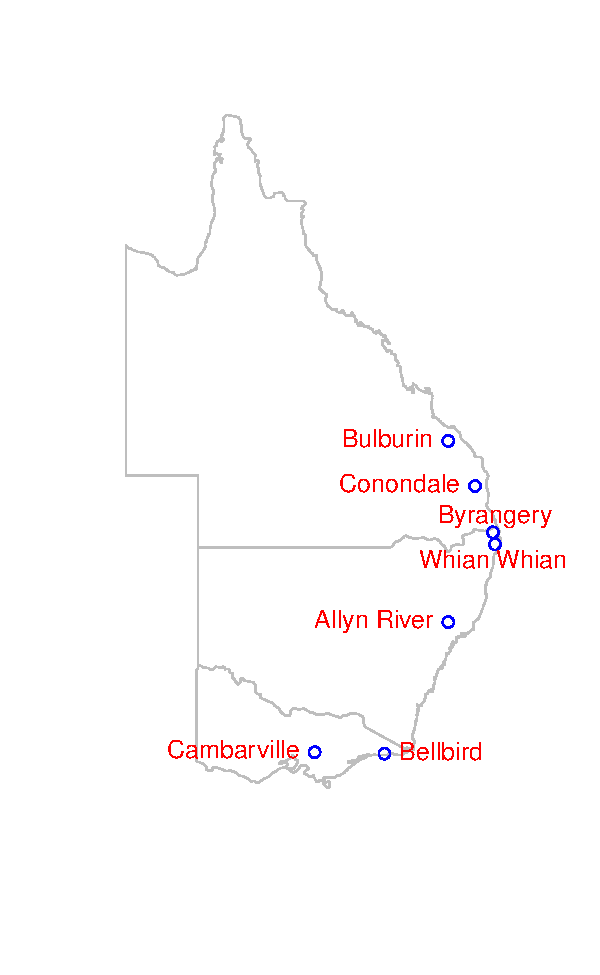
\includegraphics[width=0.6\textwidth]{figs/map-oz-sites-13_1-1} 

}



\end{knitrout}

\caption{Sites at which possums were collected.\label{fig:possumsites}}
\end{figure}



\begin{knitrout}
\definecolor{shadecolor}{rgb}{0.969, 0.969, 0.969}\color{fgcolor}\begin{kframe}
\begin{alltt}
\hlstd{supp13.1} \hlkwb{<-} \hlkwa{function}\hlstd{()\{}
\hlkwa{if}\hlstd{(}\hlopt{!}\hlkwd{require}\hlstd{(dismo))}\hlkwd{stop}\hlstd{(}\hlstr{'dismo must be installed'}\hlstd{)}
\hlcom{## ---- google-possums ----}
\hlcom{## Extend longitude & latitude ranges slightly}
\hlstd{lonlat} \hlkwb{<-} \hlkwd{with}\hlstd{(DAAG}\hlopt{::}\hlstd{possumsites,}
               \hlkwd{c}\hlstd{(}\hlkwd{range}\hlstd{(Longitude)}\hlopt{+}\hlkwd{c}\hlstd{(}\hlopt{-}\hlnum{3}\hlstd{,}\hlnum{3}\hlstd{),}
                 \hlkwd{range}\hlstd{(Latitude)}\hlopt{+}\hlkwd{c}\hlstd{(}\hlopt{-}\hlnum{2}\hlstd{,}\hlnum{2}\hlstd{))}
\hlstd{)}
\hlcom{## Obtain map, as a ``RasterLayer'' object}
\hlstd{googmap} \hlkwb{<-} \hlkwd{gmap}\hlstd{(}\hlkwd{extent}\hlstd{(lonlat))}
\hlkwd{plot}\hlstd{(googmap,} \hlkwc{inter}\hlstd{=}\hlnum{TRUE}\hlstd{)}
\hlcom{## From latitude/longitude to Mercator projection}
\hlstd{xy} \hlkwb{<-} \hlkwd{Mercator}\hlstd{(}\hlkwd{with}\hlstd{(DAAG}\hlopt{::}\hlstd{possumsites,}
                    \hlkwd{cbind}\hlstd{(Longitude, Latitude)))}
\hlcom{## Points show location of sites on the map}
\hlkwd{points}\hlstd{(xy)}
\hlcom{## Add labels that give the names}
\hlkwd{text}\hlstd{(xy,} \hlkwc{labels}\hlstd{=}\hlkwd{row.names}\hlstd{(DAAG}\hlopt{::}\hlstd{possumsites))}
\hlstd{\}}
\end{alltt}
\end{kframe}
\end{knitrout}


\begin{suppfigure}
\begin{knitrout}
\definecolor{shadecolor}{rgb}{0.969, 0.969, 0.969}\color{fgcolor}\begin{kframe}
\begin{alltt}
\hlkwd{supp13.1}\hlstd{()}
\end{alltt}
\end{kframe}

{\centering 
\includegraphics[width=0.47\textwidth]{figs/map-google-possums-13_1-1} 
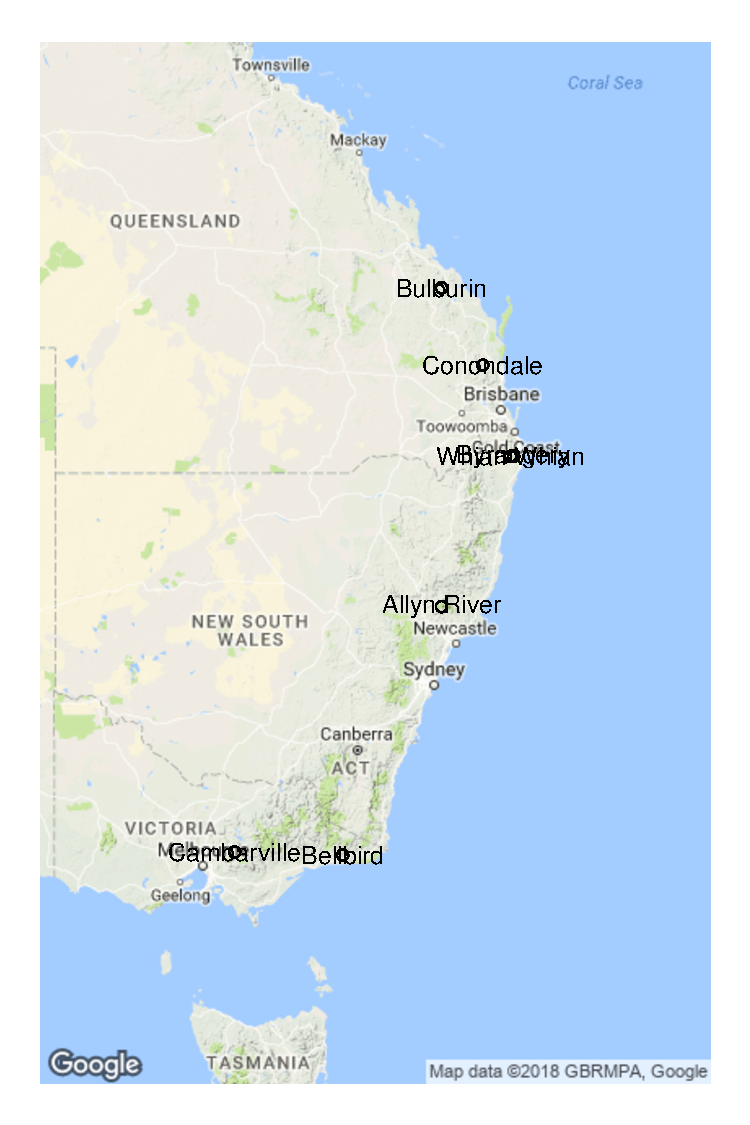
\includegraphics[width=0.47\textwidth]{figs/map-google-possums-13_1-2} 

}



\end{knitrout}
\end{suppfigure}

\begin{knitrout}
\definecolor{shadecolor}{rgb}{0.969, 0.969, 0.969}\color{fgcolor}\begin{kframe}
\begin{alltt}
\hlstd{supp13.2} \hlkwb{<-} \hlkwa{function}\hlstd{()\{}
    \hlkwa{if}\hlstd{(}\hlopt{!}\hlkwd{require}\hlstd{(plotKML))}\hlkwd{stop}\hlstd{(}\hlstr{"plotKML must be installed."}\hlstd{)}
\hlcom{## ---- plotKML ----}
\hlkwd{plotKML}\hlstd{(quakes[}\hlstr{'Energy'}\hlstd{],} \hlkwc{points_names}\hlstd{=}\hlstr{""}\hlstd{)}
\hlstd{\}}
\end{alltt}
\end{kframe}
\end{knitrout}

\begin{knitrout}
\definecolor{shadecolor}{rgb}{0.969, 0.969, 0.969}\color{fgcolor}\begin{kframe}
\begin{alltt}
\hlcom{## Input data from internet}
\hlstd{from} \hlkwb{<-}
  \hlkwd{paste}\hlstd{(}\hlkwd{c}\hlstd{(}\hlstr{"http://wfs-beta.geonet.org.nz/"}\hlstd{,}
          \hlstr{"geoserver/geonet/ows?service=WFS"}\hlstd{,}
          \hlstr{"&version=1.0.0"}\hlstd{,}
          \hlstr{"&request=GetFeature"}\hlstd{,}
          \hlstr{"&typeName=geonet:quake"}\hlstd{,}
          \hlstr{"&outputFormat=csv"}\hlstd{,}
          \hlstr{"&cql_filter=origintime%3E='2009-08-01'"}\hlstd{,}
          \hlstr{"+AND+magnitude>4.5"}\hlstd{),}
        \hlkwc{collapse}\hlstd{=}\hlstr{""}\hlstd{)}
\hlstd{quakes} \hlkwb{<-} \hlkwd{read.csv}\hlstd{(from)}
\hlstd{z} \hlkwb{<-} \hlkwd{strsplit}\hlstd{(}\hlkwd{as.character}\hlstd{(quakes}\hlopt{$}\hlstd{origintime),}
              \hlkwc{split}\hlstd{=}\hlstr{"T"}\hlstd{)}
\hlstd{quakes}\hlopt{$}\hlstd{Date} \hlkwb{<-} \hlkwd{sapply}\hlstd{(z,} \hlkwa{function}\hlstd{(}\hlkwc{x}\hlstd{)}\hlkwd{as.Date}\hlstd{(x[}\hlnum{1}\hlstd{]))}
\hlstd{quakes}\hlopt{$}\hlstd{Time} \hlkwb{<-} \hlkwd{sapply}\hlstd{(z,} \hlkwa{function}\hlstd{(}\hlkwc{x}\hlstd{)x[}\hlnum{2}\hlstd{])}
\hlstd{quakes}\hlopt{$}\hlstd{Energy} \hlkwb{<-} \hlnum{10}\hlopt{^}\hlstd{quakes}\hlopt{$}\hlstd{magnitude}\hlopt{/}\hlnum{1000000}
  \hlcom{# Will make circles area proportional to Energy}
\end{alltt}
\end{kframe}
\end{knitrout}

\begin{knitrout}
\definecolor{shadecolor}{rgb}{0.969, 0.969, 0.969}\color{fgcolor}\begin{kframe}
\begin{alltt}
\hlcom{## Prepare data for plotting}
\hlkwd{coordinates}\hlstd{(quakes)} \hlkwb{<-} \hlopt{~} \hlstd{longitude}\hlopt{+}\hlstd{latitude}
\hlkwd{proj4string}\hlstd{(quakes)} \hlkwb{<-}
  \hlkwd{CRS}\hlstd{(}\hlstr{"+proj=longlat +datum=WGS84"}\hlstd{)}
\end{alltt}
\end{kframe}
\end{knitrout}

\begin{suppfigure}
\begin{knitrout}
\definecolor{shadecolor}{rgb}{0.969, 0.969, 0.969}\color{fgcolor}\begin{kframe}
\begin{alltt}
\hlcom{## Input data from internet}
\hlstd{from} \hlkwb{<-}
  \hlkwd{paste}\hlstd{(}\hlkwd{c}\hlstd{(}\hlstr{"http://wfs-beta.geonet.org.nz/"}\hlstd{,}
          \hlstr{"geoserver/geonet/ows?service=WFS"}\hlstd{,}
          \hlstr{"&version=1.0.0"}\hlstd{,}
          \hlstr{"&request=GetFeature"}\hlstd{,}
          \hlstr{"&typeName=geonet:quake"}\hlstd{,}
          \hlstr{"&outputFormat=csv"}\hlstd{,}
          \hlstr{"&cql_filter=origintime%3E='2009-08-01'"}\hlstd{,}
          \hlstr{"+AND+magnitude>4.5"}\hlstd{),}
        \hlkwc{collapse}\hlstd{=}\hlstr{""}\hlstd{)}
\hlstd{quakes} \hlkwb{<-} \hlkwd{read.csv}\hlstd{(from)}
\hlstd{z} \hlkwb{<-} \hlkwd{strsplit}\hlstd{(}\hlkwd{as.character}\hlstd{(quakes}\hlopt{$}\hlstd{origintime),}
              \hlkwc{split}\hlstd{=}\hlstr{"T"}\hlstd{)}
\hlstd{quakes}\hlopt{$}\hlstd{Date} \hlkwb{<-} \hlkwd{sapply}\hlstd{(z,} \hlkwa{function}\hlstd{(}\hlkwc{x}\hlstd{)}\hlkwd{as.Date}\hlstd{(x[}\hlnum{1}\hlstd{]))}
\hlstd{quakes}\hlopt{$}\hlstd{Time} \hlkwb{<-} \hlkwd{sapply}\hlstd{(z,} \hlkwa{function}\hlstd{(}\hlkwc{x}\hlstd{)x[}\hlnum{2}\hlstd{])}
\hlstd{quakes}\hlopt{$}\hlstd{Energy} \hlkwb{<-} \hlnum{10}\hlopt{^}\hlstd{quakes}\hlopt{$}\hlstd{magnitude}\hlopt{/}\hlnum{1000000}
  \hlcom{# Will make circles area proportional to Energy}
\hlcom{## Prepare data for plotting}
\hlkwd{coordinates}\hlstd{(quakes)} \hlkwb{<-} \hlopt{~} \hlstd{longitude}\hlopt{+}\hlstd{latitude}
\hlkwd{proj4string}\hlstd{(quakes)} \hlkwb{<-}
  \hlkwd{CRS}\hlstd{(}\hlstr{"+proj=longlat +datum=WGS84"}\hlstd{)}
\hlkwd{supp13.2}\hlstd{()}
\end{alltt}
\end{kframe}
\end{knitrout}
\end{suppfigure}

\begin{knitrout}
\definecolor{shadecolor}{rgb}{0.969, 0.969, 0.969}\color{fgcolor}\begin{kframe}
\begin{alltt}
\hlcom{## ---- logofile ----}
\hlstd{logofile} \hlkwb{<-} \hlkwd{system.file}\hlstd{(}\hlstr{"pictures/Rlogo.jpg"}\hlstd{,}
                        \hlkwc{package} \hlstd{=} \hlstr{"rgdal"}\hlstd{)[}\hlnum{1}\hlstd{]}
\hlstd{rlogo} \hlkwb{<-} \hlstd{rgdal}\hlopt{::}\hlkwd{readGDAL}\hlstd{(logofile,} \hlkwc{silent}\hlstd{=}\hlnum{TRUE}\hlstd{)}
\end{alltt}


{\ttfamily\noindent\color{warningcolor}{Warning in rgdal::readGDAL(logofile, silent = TRUE): GeoTransform values not available}}\begin{alltt}
\hlstd{fig13.2} \hlkwb{<-} \hlkwa{function}\hlstd{()\{}
\hlcom{## ---- rlogo-image ----}
\hlkwd{image}\hlstd{(rlogo,} \hlkwc{red}\hlstd{=}\hlstr{"band1"}\hlstd{,}
      \hlkwc{green}\hlstd{=}\hlstr{"band2"}\hlstd{,}
      \hlkwc{blue}\hlstd{=}\hlstr{"band3"}\hlstd{)}
\hlstd{\}}
\end{alltt}
\end{kframe}
\end{knitrout}

\begin{figure}
\begin{knitrout}
\definecolor{shadecolor}{rgb}{0.969, 0.969, 0.969}\color{fgcolor}\begin{kframe}
\begin{alltt}
\hlkwd{fig13.2}\hlstd{()}
\end{alltt}
\end{kframe}

{\centering 
\includegraphics[width=0.47\textwidth]{figs/map-rlogo-image-13_2-1} 

}



\end{knitrout}
\caption{The function \txtt{image()} has been used to display the R
  logo image that had been input as a GDAL grid map.\label{fig:rlogo}}
\end{figure}

\begin{knitrout}
\definecolor{shadecolor}{rgb}{0.969, 0.969, 0.969}\color{fgcolor}\begin{kframe}
\begin{alltt}
\hlstd{fig13.3} \hlkwb{<-} \hlkwa{function}\hlstd{()\{}
\hlcom{## ---- spplot-col3 ----}
\hlcom{## Code}
\hlstd{col3} \hlkwb{<-} \hlkwd{c}\hlstd{(}\hlstr{"red"}\hlstd{,}\hlstr{"green"}\hlstd{,}\hlstr{"blue"}\hlstd{)}
\hlkwd{spplot}\hlstd{(rlogo,} \hlkwc{zcol}\hlstd{=}\hlnum{1}\hlopt{:}\hlnum{3}\hlstd{,} \hlkwc{names.attr}\hlstd{=col3,}
       \hlkwc{col.regions}\hlstd{=}\hlkwd{grey}\hlstd{(}\hlnum{0}\hlopt{:}\hlnum{100}\hlopt{/}\hlnum{100}\hlstd{),} \hlkwc{as.table}\hlstd{=}\hlnum{TRUE}\hlstd{,}
       \hlkwc{layout}\hlstd{=}\hlkwd{c}\hlstd{(}\hlnum{3}\hlstd{,}\hlnum{1}\hlstd{),} \hlkwc{main}\hlstd{=}\hlkwd{paste}\hlstd{(}\hlstr{"3-layer (RGB)"}\hlstd{,}
       \hlstr{"raster image - example"}\hlstd{))}
\hlstd{\}}
\end{alltt}
\end{kframe}
\end{knitrout}

\begin{figure}
\begin{knitrout}
\definecolor{shadecolor}{rgb}{0.969, 0.969, 0.969}\color{fgcolor}

{\centering 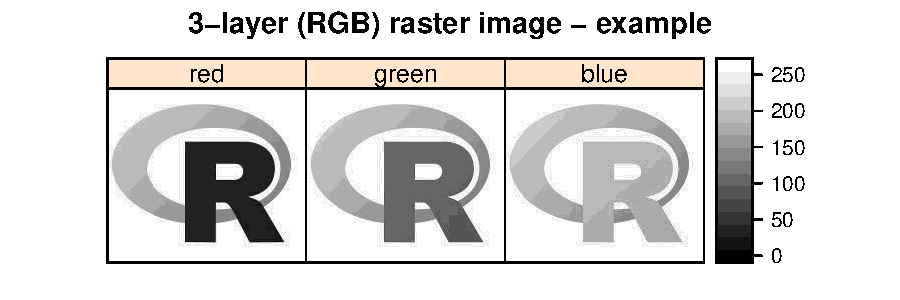
\includegraphics[width=\maxwidth]{figs/map-spplot-col3-13_3-1} 

}



\end{knitrout}
\caption{Red, green and blue layers from the R logo image.\label{fig:rlogo3}}
\end{figure}

\begin{knitrout}
\definecolor{shadecolor}{rgb}{0.969, 0.969, 0.969}\color{fgcolor}\begin{kframe}
\begin{alltt}
\hlstd{supp13.3} \hlkwb{<-} \hlkwa{function}\hlstd{()\{}
\hlcom{## ---- sp27 ----}
\hlstd{sp27} \hlkwb{<-} \hlkwd{system.file}\hlstd{(}\hlstr{"pictures/SP27GTIF.TIF"}\hlstd{,}
                    \hlkwc{package} \hlstd{=} \hlstr{"rgdal"}\hlstd{)[}\hlnum{1}\hlstd{]}
\hlcom{## ---- sp27-read ----}
\hlstd{SP27GTIF} \hlkwb{<-} \hlstd{rgdal}\hlopt{::}\hlkwd{readGDAL}\hlstd{(sp27,} \hlkwc{output.dim}\hlstd{=}\hlkwd{c}\hlstd{(}\hlnum{100}\hlstd{,}\hlnum{100}\hlstd{),}
                     \hlkwc{silent}\hlstd{=}\hlnum{TRUE}\hlstd{)}
\hlkwd{class}\hlstd{(SP27GTIF)}
\hlcom{## ---- sp27-spplot ----}
\hlkwd{spplot}\hlstd{(SP27GTIF)}
\hlstd{\}}
\end{alltt}
\end{kframe}
\end{knitrout}

\begin{suppfigure}
\begin{knitrout}
\definecolor{shadecolor}{rgb}{0.969, 0.969, 0.969}\color{fgcolor}\begin{kframe}
\begin{alltt}
\hlkwd{supp13.3}\hlstd{()}
\end{alltt}
\end{kframe}

{\centering 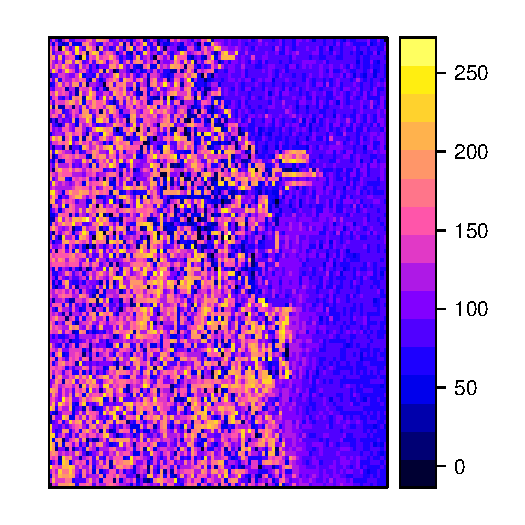
\includegraphics[width=0.6\textwidth]{figs/map-sp27-13_3-1} 

}



\end{knitrout}
\end{suppfigure}



\begin{knitrout}
\definecolor{shadecolor}{rgb}{0.969, 0.969, 0.969}\color{fgcolor}\begin{kframe}
\begin{alltt}
\hlstd{fig13.4} \hlkwb{<-} \hlkwa{function}\hlstd{()\{}
\hlcom{## ---- meuse-bubble ----}
\hlkwd{data}\hlstd{(meuse);} \hlkwd{data}\hlstd{(meuse.riv)}
\hlkwd{coordinates}\hlstd{(meuse)} \hlkwb{<-} \hlopt{~} \hlstd{x} \hlopt{+} \hlstd{y}
\hlstd{gph} \hlkwb{<-} \hlkwd{bubble}\hlstd{(meuse,} \hlstr{"zinc"}\hlstd{,} \hlkwc{pch}\hlstd{=}\hlnum{1}\hlstd{,}
              \hlkwc{key.entries} \hlstd{=}  \hlnum{100} \hlopt{*} \hlnum{2}\hlopt{^}\hlstd{(}\hlnum{0}\hlopt{:}\hlnum{4}\hlstd{),}
              \hlkwc{main} \hlstd{=} \hlstr{"Zinc(ppm)"}\hlstd{,}
              \hlkwc{scales}\hlstd{=}\hlkwd{list}\hlstd{(}\hlkwc{axes}\hlstd{=}\hlnum{TRUE}\hlstd{,} \hlkwc{tck}\hlstd{=}\hlnum{0.4}\hlstd{))}
\hlstd{add} \hlkwb{<-}
  \hlstd{latticeExtra}\hlopt{::}\hlkwd{layer}\hlstd{(}\hlkwd{panel.lines}\hlstd{(meuse.riv[,}\hlnum{1}\hlstd{],}
                                  \hlstd{meuse.riv[,}\hlnum{2}\hlstd{],}
                      \hlkwc{col}\hlstd{=}\hlstr{"gray"}\hlstd{))}
\hlstd{gph}\hlopt{+}\hlstd{add}
\hlstd{\}}
\end{alltt}
\end{kframe}
\end{knitrout}

\begin{figure}
\begin{knitrout}
\definecolor{shadecolor}{rgb}{0.969, 0.969, 0.969}\color{fgcolor}\begin{kframe}
\begin{alltt}
\hlkwd{fig13.4}\hlstd{()}
\end{alltt}
\end{kframe}

{\centering 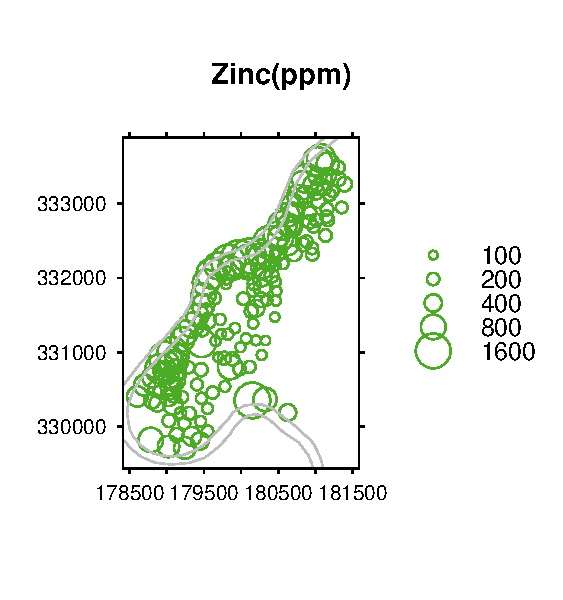
\includegraphics[width=0.47\textwidth]{figs/map-meuse-bubble-13_4-1} 

}



\end{knitrout}
 \caption{Bubble plot for \txtt{zinc},
with area of bubbles proportional to concentration.
River Meuse boundaries are in gray.\label{fig:ZnRiv}}
\end{figure}

\begin{knitrout}
\definecolor{shadecolor}{rgb}{0.969, 0.969, 0.969}\color{fgcolor}\begin{kframe}
\begin{alltt}
\hlstd{supp13.4} \hlkwb{<-} \hlkwa{function}\hlstd{()\{}
\hlcom{## ---- show-shape ----}
\hlstd{dsn} \hlkwb{<-} \hlkwd{system.file}\hlstd{(}\hlstr{"vectors"}\hlstd{,} \hlkwc{package} \hlstd{=} \hlstr{"rgdal"}\hlstd{)[}\hlnum{1}\hlstd{]}
\hlcom{## ---- shape-in ----}
\hlstd{cities} \hlkwb{<-} \hlstd{rgdal}\hlopt{::}\hlkwd{readOGR}\hlstd{(}\hlkwc{dsn}\hlstd{=dsn,} \hlkwc{layer}\hlstd{=}\hlstr{"cities"}\hlstd{,} \hlkwc{verbose}\hlstd{=}\hlnum{FALSE}\hlstd{)}
\hlcom{## ---- canada-plot ----}
\hlstd{canada} \hlkwb{<-} \hlkwd{subset}\hlstd{(cities, COUNTRY}\hlopt{==}\hlstr{"Canada"}\hlstd{)}
\hlkwd{trellis.par.set}\hlstd{(}\hlkwd{sp.theme}\hlstd{())}
\hlkwd{spplot}\hlstd{(cities,} \hlkwc{zcol}\hlstd{=}\hlstr{"POPULATION"}\hlstd{)}
\hlstd{\}}
\end{alltt}
\end{kframe}
\end{knitrout}

\begin{suppfigure}
\begin{knitrout}
\definecolor{shadecolor}{rgb}{0.969, 0.969, 0.969}\color{fgcolor}\begin{kframe}
\begin{alltt}
\hlkwd{supp13.4}\hlstd{()}
\end{alltt}
\end{kframe}

{\centering 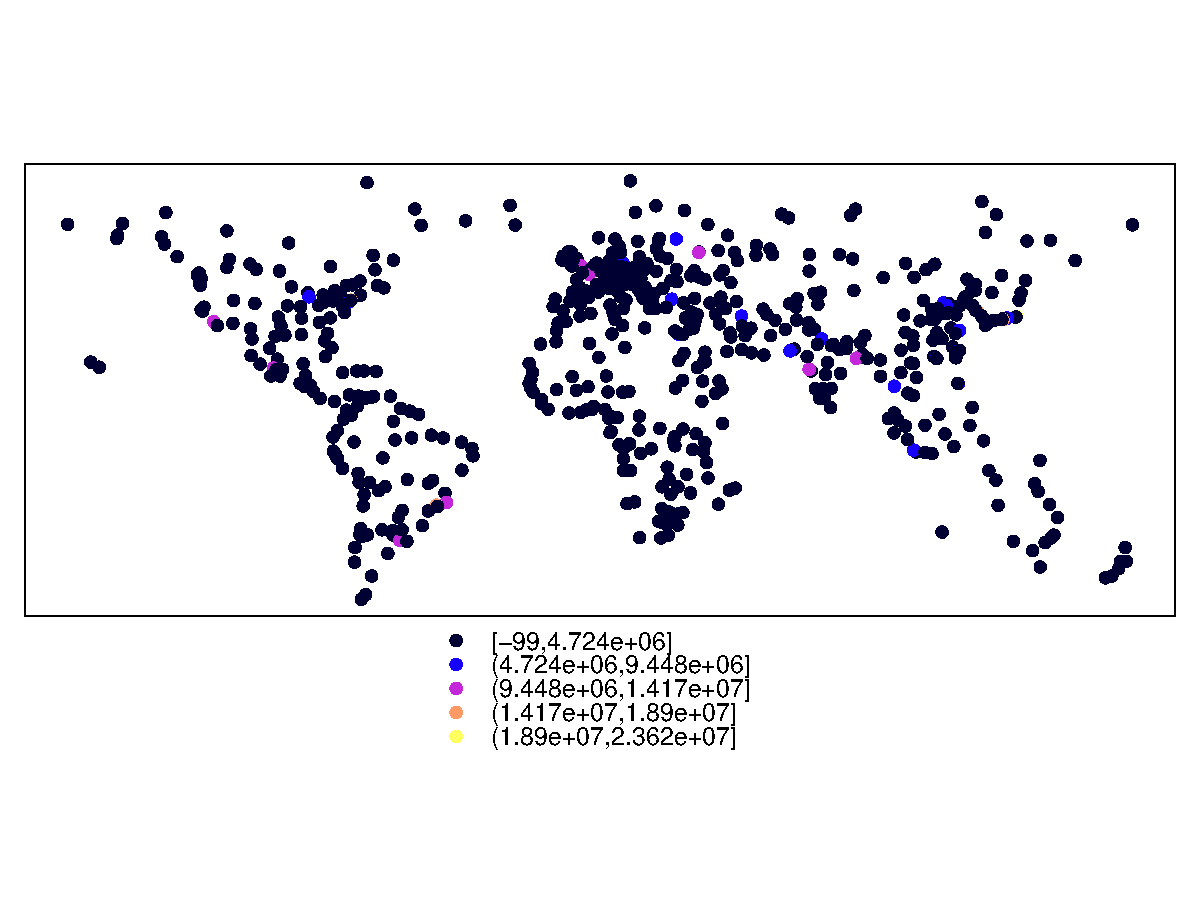
\includegraphics[width=0.97\textwidth]{figs/map-shape-supp13_4-1} 

}



\end{knitrout}
\caption{Plot derived from shapefile information.}
\end{suppfigure}

\end{document}


